%%% Copyright page
\clearpage
\thispagestyle{fancy}

\fancyhf{} % remove everything
\renewcommand{\headrulewidth}{0pt} % remove lines as well
\renewcommand{\footrulewidth}{0pt}

\vspace*{\fill}


\begin{center}
\includegraphics[width=100pt]{by-nc-sa.eps}
\end{center}

\begin{center}
\emph{Stuff Goes Bad: Erlang in Anger} by Fred Hébert and Heroku is licensed under a \href{http://creativecommons.org/licenses/by-nc-sa/4.0/}{Creative Commons Attribution-NonCommercial-ShareAlike 4.0 International License}.
\end{center}

Thanks for the additional work, reviewing, and/or editing done by:

\emph{Jacob Vorreuter}, \emph{Seth Falcon}, \emph{Raoul Duke}, \emph{Nathaniel Waisbrot}, \emph{David Holland}, \emph{Alisdair Sullivan}, \emph{Lukas Larsson}, \emph{Tim Chevalier}, \emph{Paul Bone}, \emph{Jonathan Roes}, \emph{Roberto Aloi}, \emph{Dmytro Lytovchenko}, and \emph{Tristan Sloughter}.

\null
\vfill
%\vspace*{\fill}
The cover image is a modified version of \href{http://www.freeimages.com/photo/533163}{fallout shelter} by \href{http://www.freeimages.com/profile/drouu}{drouu} on \href{http://sxc.hu}{sxc.hu}.
\cfoot{\emph{v1.1.0}}
\rfoot{\emph{2016-04-06}}


%% License as of Monday, August 18, 2014:
%%
%% you may use any of my photos, original or modified, for any purpose whatsoever (personal, non-profit, or commercial; for web or print). you do not need to contact me prior to or after using one of my photos, though a comment or note is always appreciated if you have the opportunity.
%%
%% you may not claim ownership or copyright of my photos. seriously, i have an orbital karma gun and i'm not afraid to use it.
